 % Theory of elasticity and failure
 \chapter{Elasticity and failure}
 To have a framework to discuss failure and fracture in methane hydrates, I will introduce some theory of elasticity and failure in linear elastic materials. This will also be needed in order to be explicit about how stresses and strains are imposed on the model systems.

 \section{Linear elasticity}
In general, methane hydrates are anisotropic materials. However, they are sufficiently isotropic to be treated as isotropic in this work. I will start by introducing the general tensor form of Hooke's law , and then provide the simplifications resulting from looking at an isotropic material. This presentation will take Hooke's law as a given, but it can be derived for example with an energy approach as in \citet[p.105]{Buehler2008}.

\subsection{Stress and strain}
Linear elasticity is based on the idea that deformations on a material will result in a linear reaction in terms of forces from that material. \emph{Strain}, $\epsilon$, is a deformation, and the \emph{normal} strain is defined as the relative elongation of a body;
\begin{equation}
	\epsilon = \frac{l-l_0}{l_0}
\end{equation}
Where $l_0$ is the equilibrium length of that body and $l$ is the final length. Additionally, the body can be subjected to \emph{shear strain}. Shear strain can be defined as the in-plane component of the difference in midpoint position between two facing end planes of an infinitesimal cubic element divided by the equilibrium distance between these planes.

It is common to use an index notation that clarifies on what plane a strain is present, and in which direction. Strains are denoted $\epsilon_{ij}$ where the first index says what planes are involved in the strain (the index denotes a vector perpendicular to the plane), and the second index says in what direction the strain is present. For instance: $\epsilon_{yy}$ is the relative elongation of the distance between the $xz$ end-planes of an infinitesimal cubic element, whereas $\epsilon_{xy}$ is the $y$-component of the distance between the midpoint of the left and right $yz$-planes divided by the $x$-component of the equilibrium distance between these points.

\emph{Stress} is a force density acting on a body. Uniform normal stress on a plane is defined as:
\begin{equation}
	\sigma_n = \frac{F_\perp}{A}
\end{equation}
Shear stress is the force parallel to the plane:
\begin{equation}
	\sigma_s = \frac{F_\parallel}{A}
\end{equation}

Like for strains, stress on different planes and directions of an infinitesimal cube are indexed like $\sigma_{ij}$ where $i$ says what plane the force acts in, and $j$ in what direction the force acts.

\subsection{Hooke's law}
Stresses cause strains and vice versa. This is reflected in the generalized Hooke's law:
\begin{equation}
	\sigma_{ij} = c_{ijkl}\epsilon_{kl}
\end{equation}
This law relates the Cauchy stress tensor $\sigma_{ij}$ to the strain tensor $\epsilon_{kl}$ in a linearly elastic material. All material properties are contained in the stiffness tensor $c_{ijkl}$.
In this form, Hooke's law basically states that each component of the Cauchy stress tensor depends linearly on \emph{all} components of the strain tensor. 

Hooke's law contains two tensors of rank 2 with 9 components each, and one tensor of rank 4 with 81 components. Fortunately, there are symmetries to be exploited. First, the Cauchy stress tensor is symmetric, which leads to $c_{ijkl} = c_{jikl}$. Second, the strain tensor is symmetric, so $c_{ijkl} = c_{ijlk}$. This means we are left with 6 independent combinations of each of $ij$ and $kl$, and a total of 36 components. 

Using the rank reduction method of Voigt (\cite{voigt1928lehrbuch}, or any standard book on elasticity), the stress and strain matrices can be written as vectors:
\begin{equation}
	\uline{\sigma} = 
	\begin{pmatrix}
	\sigma_{11} & \sigma_{12} & \sigma_{13} \\
	\sigma_{21} & \sigma_{22} & \sigma_{23} \\
	\sigma_{31} & \sigma_{32} & \sigma_{33} \\ 
	\end{pmatrix}
	\to 
	\vec{\sigma} = 
	\begin{pmatrix}
	\sigma_{11} \\ \sigma_{22} \\ \sigma_{33} \\ \sigma_{23} \\ \sigma_{13} \\ \sigma_{12}
	\end{pmatrix}
	\equiv
	\begin{pmatrix}
	\sigma_{1} \\ \sigma_{2} \\ \sigma_{3} \\ \sigma_{4} \\ \sigma_{5} \\ \sigma_{6}
	\end{pmatrix}
	\label{eq:sigma_def}
\end{equation}

\begin{equation}
	\uline{\epsilon} = 
	\begin{pmatrix}
	\epsilon_{11} & \epsilon_{12} & \epsilon_{13} \\
	\epsilon_{21} & \epsilon_{22} & \epsilon_{23} \\
	\epsilon_{31} & \epsilon_{32} & \epsilon_{33} \\ 
	\end{pmatrix}
	\to 
	\vec{\epsilon} = 
	\begin{pmatrix}
	\epsilon_{11} \\ \epsilon_{22} \\ \epsilon_{33} \\ 2\epsilon_{23} \\ 2\epsilon_{13} \\ 2\epsilon_{12}
	\end{pmatrix}
	\equiv
	\begin{pmatrix}
	\epsilon_{1} \\ \epsilon_{2} \\ \epsilon_{3} \\ \epsilon_{4} \\ \epsilon_{5} \\ \epsilon_{6}
	\end{pmatrix}
	\label{eq:epsilon_def}
\end{equation}
For the same reasons, the stiffness tensor can be reduced to rank 2 (I choose not to write out the complete stiffness tensor, only the reduced one):
\begin{equation}
	\vec{C} =
	\begin{pmatrix}
	C_{11} & C_{12} & C_{13} & C_{14} & C_{15} & C_{16} \\
	C_{21} & C_{22} & C_{23} & C_{24} & C_{25} & C_{26} \\
	C_{31} & C_{31} & C_{33} & C_{34} & C_{35} & C_{36} \\
	C_{41} & C_{42} & C_{43} & C_{44} & C_{45} & C_{46} \\
	C_{51} & C_{52} & C_{53} & C_{54} & C_{55} & C_{56} \\
	C_{61} & C_{62} & C_{63} & C_{64} & C_{65} & C_{66}
	\end{pmatrix}
\end{equation}
Hooke's law can now be written as a matrix equation:
\begin{equation}
	\vec{\sigma} = \vec{C}\vec{\epsilon}
\end{equation}
It actually turns out that the stiffness matrix is symmetric, because stress and strain are work-conjugates:
\begin{equation}
	\sigma_i = \frac{\partial u}{\partial \epsilon_i}
\end{equation}
Where $u$ is the energy volume density associated with the stress-strain configuration.
Inserting this into Hooke's law gives:
\begin{equation}
	C_{ij}=\frac{\partial^2 u}{\partial \epsilon_i \partial \epsilon_j} = \frac{1}{V} \frac{\partial^2 U}{\partial \epsilon_i \partial \epsilon_j} 
\end{equation}
This relation can be used to calculate the stiffness matrix from any simulation of an elastic material where strains can be imposed and potential energy can be measured.

When representing the stress and strain matrices in practice, it is common to distinguish between stress and strain contributions. In standard Cartesian coordinates, equations \ref{eq:sigma_def} and \ref{eq:epsilon_def} turn into:
\begin{equation}
	\uline{\sigma} = 
	\begin{pmatrix}
	\sigma_{xx} & \tau_{xy} & \tau_{xz} \\
	\tau_{yx} & \sigma_{yy} & \tau_{yz} \\
	\tau_{zx} & \tau_{zy} & \sigma_{zz} \\ 
	\end{pmatrix}
	\to 
	\vec{\sigma} = 
	\begin{pmatrix}
	\sigma_{xx} \\ \sigma_{yy} \\ \sigma_{zz} \\ \tau_{yz} \\ \tau_{xz} \\ \tau_{xy}
	\end{pmatrix}
\end{equation}

\begin{equation}
	\uline{\epsilon} = 
	\begin{pmatrix}
	\epsilon_{xx} & \epsilon_{xy} & \epsilon_{xz} \\
	\epsilon_{yx} & \epsilon_{yy} & \epsilon_{yz} \\
	\epsilon_{zx} & \epsilon_{zy} & \epsilon_{zz} \\ 
	\end{pmatrix}
	\to 
	\vec{\epsilon} = 
	\begin{pmatrix}
	\epsilon_{xx} \\ \epsilon_{yy} \\ \epsilon_{zz} \\ \epsilon_{yz} \\ \epsilon_{xz} \\ \epsilon_{xy}
	\end{pmatrix}
\end{equation}
Where the shear stress components have changed from $\sigma$ to $\tau$. This is the notation I will use.

\subsection{Isotropic materials}
An isotropic material is a material where the stiffness properties does not depend on space directions in the material. Isotropic materials can be described by two independent parameters, for example Young's modulus $E$ and Poisson's ratio $\nu$. 
Young's modulus can be defined as:
\begin{equation}
	E = \frac{\sigma_{xx}}{\epsilon_{xx}}
\end{equation}
Where $\sigma_{xx}$ is a normal stress applied in the same direction as the normal strain $\epsilon_{xx}$ is measured. This strain is known as \emph{normal strain}. Since the directions don't matter in isotropic materials, I have chosen to define Young's modulus along the x-axis. When an isotropic material is subjected to tensile stress, and becomes longer, it will simultaneously contract in the directions normal to the applied tension. This is known as \emph{lateral strain}. The ratio of lateral strain to normal strain is known as \emph{Poisson's ratio}:
\begin{equation}
	\nu = -\frac{\epsilon_{yy}}{\epsilon_{xx}} = -\frac{\epsilon_{zz}}{\epsilon_{xx}}
\end{equation}
As promised, these two properties shall completely describe the elastic material. The stiffness tensor of an isotropic material is:
\begin{equation}
	\vec{C} = 
   	\frac{E}{(1+\nu)(1-2\nu)}
   	\begin{pmatrix}
		1-\nu & \nu & \nu & 0 & 0 & 0 \\
		\nu & 1-\nu & \nu & 0 & 0 & 0 \\
		   \nu & \nu & 1-\nu & 0 & 0 & 0 \\
		   0 & 0 & 0 & (1-2\nu)/2 & 0 & 0 \\
		   0 & 0 & 0 & 0 & (1-2\nu)/2 & 0 \\
		   0 & 0 & 0 & 0 & 0 & (1-2\nu)/2
	\end{pmatrix}
\end{equation}

\subsection{Plane strain and plane stress}
There are conditions where a three-dimensional elastic problem can be analyzed as a two-dimensional problem. This is useful for example when applying standard results of linear elastic fracture mechanics, since many of those results are for two-dimensional systems. Plane strain and plane stress are such conditions. The formal definitions of plane strain and plane stress are given in equations \ref{eq:plane_strain} and \ref{eq:plane_stress}, respectively.

\begin{equation}
\uuline \epsilon = 
\begin{pmatrix}
	\epsilon_{11} & \epsilon_{12} & 0 \\
	\epsilon_{21} & \epsilon_{22} & 0 \\
	0 & 0 & 0
\end{pmatrix}
\label{eq:plane_strain}
\end{equation}

\begin{equation}
\uuline \sigma = 
\begin{pmatrix}
	\sigma_{11} & \sigma_{12} & 0 \\
	\sigma_{21} & \sigma_{22} & 0 \\
	0 & 0 & 0
\end{pmatrix}
\label{eq:plane_stress}
\end{equation}

For plane strain, we allow a nonzero stress component $\sigma_{33}$. Likewise, for plane stress we allow a nonzero strain component $\epsilon_{33}$. However, these components can only be results of the analysis, they shall not enter the analysis. 

\subsection{Elastic moduli}
As mentioned earlier, an isotropic material can be uniquely described by two constants. They can for example be two of the following (there are other possible constants):
\begin{itemize}
\item Bulk modulus, $K$
\item Young's modulus, $E$
\item Lamé's first parameter, $\lambda$
\item Shear modulus, $G$
\item Poisson's ratio, $\nu$
\item P-wave modulus, $M$
\end{itemize}
Below, I write the definitions of bulk modulus and shear modulus and give their relation to Young's modulus and Poisson's ratio, as this is useful to calculate elastic wave velocities in materials.

The shear modulus is defined as the ratio of shear stress to shear strain:
\begin{equation}
	G = \frac{\sigma_{ij}}{\epsilon_{ij}}, \qquad i\neq j
\end{equation}
The shear modulus can be related to Young's modulus and Poisson's ratio by:
\begin{equation}
	G = \frac{E}{2(1+\nu)}
\end{equation}

The bulk modulus $K$ is defined as:
\begin{equation}
	K = \rho\frac{\dd P}{\dd \rho}
\end{equation}
Where $P$ is hydrostatic pressure, $P = \frac{1}{3} \left(\sigma_{xx}+\sigma_{yy}+\sigma_{zz}\right)$, when $\sigma_{xx} = \sigma_{yy} = \sigma_{zz}$. $\rho$ is the mass density of the material.
The bulk modulus can be related to Young's modulus and Poisson's ratio by:\begin{equation}
	K = \frac{E}{3(1-2\nu)}
\end{equation}

\subsection{Elastic waves}
In homogeneous isotropic materials, one can observe shear waves and pressure waves. Shear waves depend on the shear modulus and travel with a speed of:
\begin{equation}
	v_s = \sqrt{\frac{G}{\rho}} = \sqrt{\frac{E}{2\rho(1+\nu)}}
\end{equation}
Where $\rho$ is the mass density of the material.

Pressure waves depend on the bulk modulus and travel at a speed of:
\begin{equation}
	v_p = \sqrt{\frac{K}{\rho}} = \sqrt{\frac{E}{3\rho(1-2\nu)}}
\end{equation}

These relations can be used to find elastic properties from acoustic measurements. That is convenient if a material of unknown elastic moduli is hard to put in an apparatus for deformation. These relations are also convenient for finding elastic wave velocities from molecular dynamics simulations, as the moduli are easy to measure.


\section{Linear elastic fracture mechanics}
Linear elastic fracture mechanics (LEFM) deals with fracture in linear elastic materials. The simplest version of this theory assumes that fracture is governed by two equivalent properties: The stress intensity factor $K$, and the energy release rate $G$. Here, I introduce the background for these concepts.

\subsection{Brittle and ductile materials}
In materials science, it is common to distinguish between brittle and ductile materials. A material i brittle if it ``breaks without significant strain'' (Wikipedia, brittle). Brittleness can also be described as ``an inability to deform plastically'' \cite{benham1996mechanics}. whereas Ductility is a solid material's ability to deform plastically \cite{benham1996mechanics}. It is actually hard to come along a more satisfying definition -- ductility and brittleness seems to be the kind of knowledge that everyone in the field have, but no one writes down as an equation. Throughout this thesis, I will use the term brittle -- by which i will be meaning ideally brittle -- in two ways. First, the intuitive definition: A material is brittle if it can be elastically deformed and suddenly breaks over essentially no change in the strain applied to it. Secondly, a definition that will be clearer later in this section: A material is brittle if the strain energy needed to break it is only slightly higher than the energy needed to open the projected crack surface of the crack that is created when the material fails. An illustration of brittle and ductile fracture in terms of potential energy stored in the system during loading and failure is shown in figure \ref{fig:idealized_fracture}.

\begin{figure}
\centering
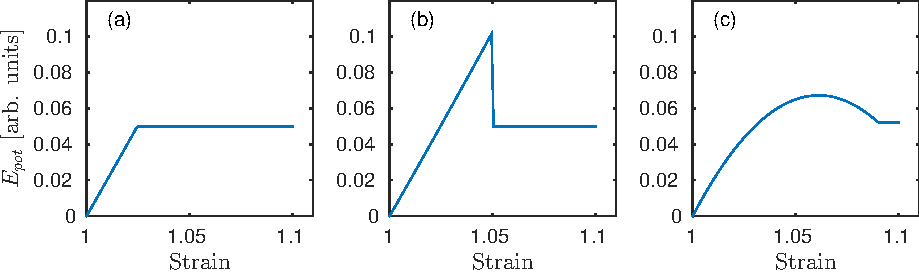
\includegraphics[width=\textwidth]{../figures/thesis/idealized_fracture_e_pot.pdf}
\caption{Potential energy as a function of applied strain for systems held at a constant temperature. The figure shows three idealized examples of failure. (a) and (b) are brittle, (c) is ductile. In (a), the system is loaded adiabatically, and reaches a stress state where $\mathcal{G}_c = 2\gamma_s$ and breaks. No energy is lost to plastic deformation or heat. In (b), the system is loaded isothermally and breaks at $\mathcal{G}_c > 2\gamma_s$. There is no plastic deformation, but heat flows in and out of the material. In (c), the system is continuously deforming plastically through the straining process -- the material is very ductile. Note that it is not possible to see the amount of energy lost to plastic deformation from (c). The plateau in all figures represents a state where a crack propagated through the whole system -- the system is divided into two parts -- so additional straining does not contribute potential energy. }
\label{fig:idealized_fracture}
\end{figure}

\subsection{Modes of loading}
There are three different modes of crack separation: I =`opening', II = `sliding', III = `tearing'. These are illustrated in figure \ref{fig:loading_modes}. The presentation from here on will only consider mode I loading -- the opening mode.

\begin{figure}
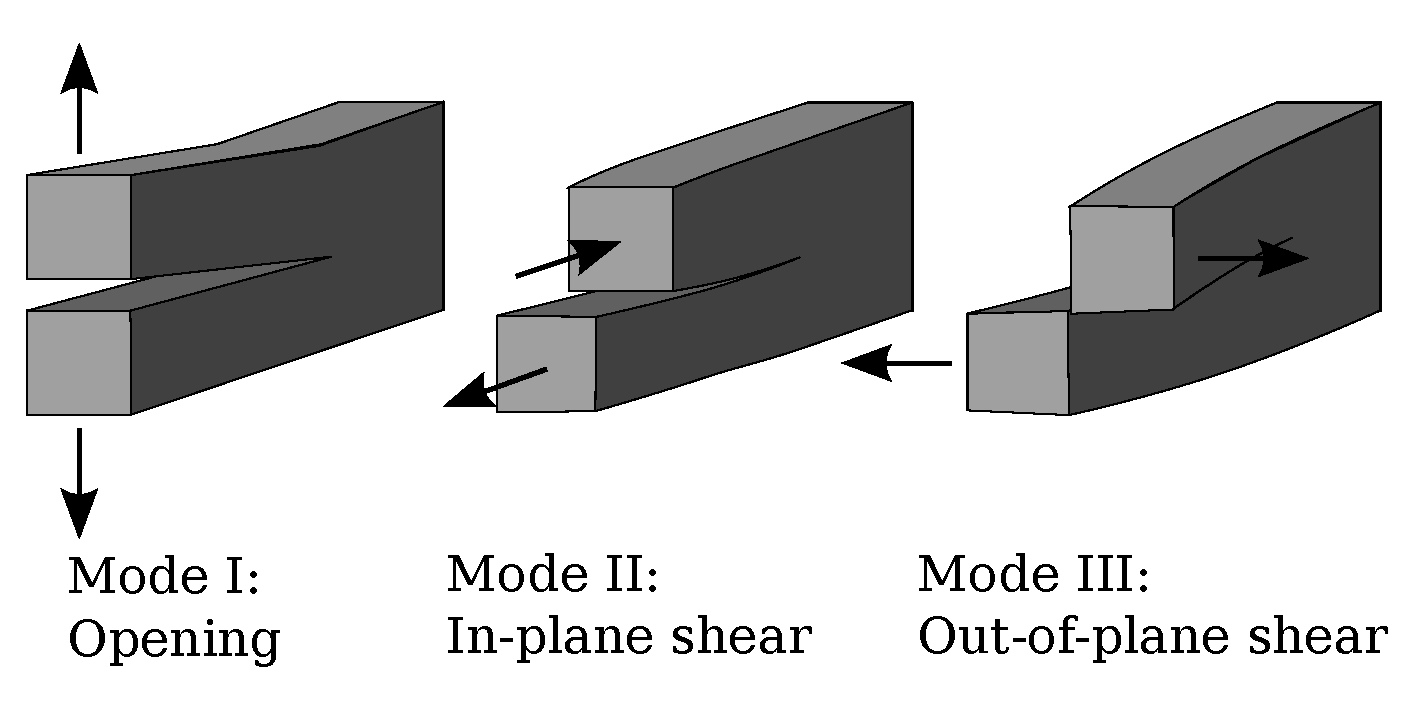
\includegraphics[width=\textwidth]{../figures/thesis/Fracture_modes_v2.pdf}
\caption{Three modes of crack separation. (``Fracture modes v2'' by Twisp. Licensed under Public Domain via Wikimedia Commons)}
\label{fig:loading_modes}
\end{figure}

\subsection{Failure criteria}
As is many fields, the first recorded studies are the ones of Leonardo da Vinci. da Vinci discovered that short iron wires are stronger than long iron wires. A common interpretation is that random flaws make the iron wires weaker at some points, and that a longer wire has a higher probability of a weak spot than a long one. More precisely: The strength will be governed by the largest flaw, and the expected size of the largest flaw grows with the wire length. A major goal of LEFM is to be able to predict the failure of structures: what is the pressure required to break a sample of a material? The first somewhat successful attempt to predict failure was the efforts of Inglis \cite{inglis1913stresses}. He introduced the concept of stress concentration at a crack tip to find the fracture toughness of brittle materials. Specifically, he found that for an elliptical crack on an infinite sheet (figure \ref{fig:elliptical_crack}, the local stress at the crack tip as a function of the faraway tensile stress was:
\begin{figure}
\centering
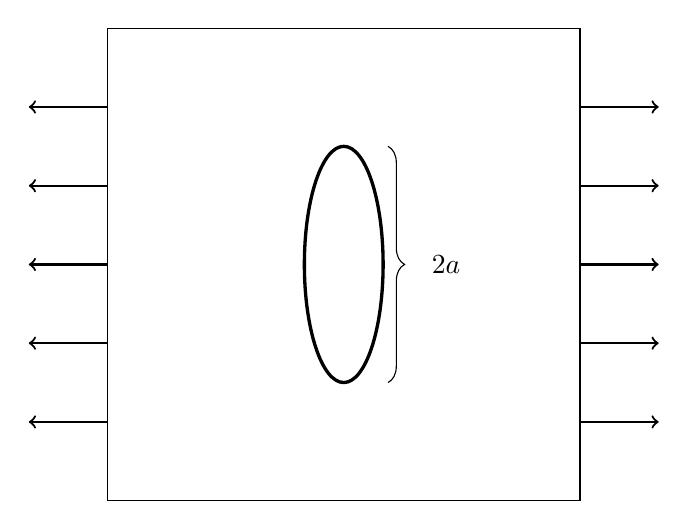
\begin{tikzpicture}
\draw  (0, 0) -- (0, 6) -- (6, 6) -- (6, 0) -- cycle;
\draw[very thick](3, 3) ellipse (0.5cm and 1.5cm);
\foreach \i in {1,2,...,5}
{
	\draw[thick,->] (0, \i) -- (-1, \i);
	\draw[thick,->] (6, \i) -- (7, \i);
}
\draw [decorate,decoration={brace,amplitude=6pt,mirror,raise=16pt},yshift=0pt]
(3 ,1.5) -- (3, 4.5) node [black,midway,xshift=1.3cm] {$2a$};
\end{tikzpicture}
\caption{Elliptical crack in an ``infinite'' plate.}
\label{fig:elliptical_crack}
\end{figure}
\begin{equation}
	\sigma_{\text{cracktip}} = 2\sigma_{\text{faraway}}\sqrt{\frac{a}{\rho}}
	\label{eq:stress_consentration}
\end{equation}
Where $a$ is half the length of the major axis of the ellipse, and $\rho$ is the radius of curvature of the ellipse close to the crack tip. The theory of Inglis is a atomistic one, and he required the stress concentration at the crack tip for failure to be the stress needed to break atomic bonds. The theory is described in \citet[p.27]{Anderson2005}. The expression for this can be found by regarding the pressure exerted between two atoms when they are dragged away from their equilibrium configuration as a sine function with a maximum stress equal to the cohesive strength $\sigma_c$ of the bond:
\begin{equation}
	\sigma = \sigma_c \sin{\frac{\pi x}{x_0}}
	\label{eq:atomic_force}
\end{equation}
Where $x_0$ is the typical distance between atoms. If the origin is set to the equilibrium distance $x_0$, and the force constrained to act for another equilibrium distance, then the energy area density to break bonds is:
\begin{equation}
u_{bond}^{area} = \int_0^{x_0} \sigma_c \sin{\frac{\pi x}{x_0}} \dd x = 2\sigma_c \frac{x_0}{\pi}
\end{equation}
It is now convenient to introduce a new quantity, the surface energy $\gamma_s$. This is the mechanical energy needed to create new crack surface area. This is exactly equal to one half of the energy area density needed to break an atomic bond, since breaking atomic bonds create two surfaces. The surface energy for this simple bond stress model is then:
\begin{equation}
	\gamma_s = \sigma_c \frac{x_0}{\pi}
	\label{eq:surface_energy}
\end{equation}

Young's modulus should (from its definition) be the slope of the stress with respect to strain. The slope of the stress with respect to distance in equation \ref{eq:atomic_force} is $\frac{\pi\sigma_c}{x_0}$, which means Young's modulus is:
\begin{equation}
E = \pi\sigma_c
\label{eq:youngs_atomistic}
\end{equation}

Combining equations \ref{eq:surface_energy} and \ref{eq:youngs_atomistic} one obtains an estimate of the cohesive strength of atom bonds using only \emph{one} atomic scale parameter, $x_0$:
\begin{equation}
	\sigma_c = \sqrt{\frac{E\gamma_s}{x_0}}
	\label{eq:critical_local}
\end{equation}
Setting the cracktip stress from equation \ref{eq:stress_consentration} equal to the critical local stress from equation \ref{eq:critical_local}, and assuming that the radius of curvature is equal to the distance between atoms (this turns out to be a good assumption, and removes the atomic scale parameter), we get an expression for the critical faraway stress level:
\begin{equation}
	\sigma_f = \sqrt{\frac{E\gamma_s}{4a}}
	\label{eq:inglis_formula}
\end{equation}
This is the Inglis formula for the fracture stress on a large sheet with a crack of width $2a$.

In 1920, Griffith improved on the flaw-approach \cite{griffith1920phenomena}, but instead of building a theory from the atomic level, he assumed the following: A crack will propagate from a flaw if the strain energy that will be released during crack growth is higher than the corresponding surface energy associated with the created crack surface. The surface energy density is denoted $\gamma_s$ and have units of energy per area. Griffith's approach works well for ideally brittle materials. The formula for critical faraway stress with Griffiths theory is:
\begin{equation}
	\sigma_f = \sqrt{\frac{2E\gamma_s}{\pi a}}
\end{equation}
For an elliptic crack of width $2a$ (Same conditions as with Inglis' theory). This expression is actually equal to the expression of Inglis, except for a factor, even though Griffith's theory is based solely on continuum mechanics.

For a sheet of finite width, the fracture stress is slightly lower, since the crack actually weakens the material (the cross sectional area bearing the stress is shrinking). The exact expression for a sheet of width $2W$ is:

 \begin{equation}
 	\sigma_f = \sqrt{\frac{2E\gamma_s}{2W\tan\left( \frac{\pi a}{2W}\right)}}
 	\label{eq:griffith_finite_sheet}
 \end{equation}

For reference, I also include the formula for the fracture stress of a penny-shaped crack subjected to remote tensile stress:
\begin{equation}
	\sigma_f = \sqrt{\frac{\pi E \gamma_s }{2(1-\nu^2)a}}
\end{equation}
 

 Irwin refined Griffith's approach, and introduced the \emph{energy release rate} rate \cite{irwin2onset}, $\mathcal{G}$. The energy release rate is a property of the elastic state of a linearly elastic material. According to Irwin, a crack will propagate when $\mathcal{G}$ becomes larger than a material-specific value $\mathcal{G}_c$ -- the \emph{critical} energy release rate. This differs from Griffith's theory, since the critical energy release rate doesn't necessarily have to be the same as the surface energy. For a straight crack of width $2a$ (no longer required to be elliptic) on an infinite plate subjected to tensile stress, the energy release rate is:

\begin{equation}
	\mathcal{G} = \frac{\pi \sigma^2 a}{E}
\end{equation}

This is purely a relation concerning how a linear elastic material distributes energy during crack opening. In the particular case of a straight crack on an infinite sheet, we see that the longer the crack, the higher the energy release rate. This fits with the intuition that a larger flaw will reduce the strength of a material. Note that the material doesn't get weaker because the flaw reduces the load-bearing area (the sheet is infinite). The material gets weaker because a longer crack increases the elastic energy that gets released per crack area grown. The critical value can be measured experimentally using a sample with an artificial flaw whose length is known, and measure the yield pressure. 

Notice that the formula for energy release rate is actually equivalent to the Griffith formula, equation \ref{eq:griffith_finite_sheet}, except that the surface energy $2\gamma_s$ is swapped with the energy release rate.

Irwin also introduced another property, which is equivalent to the energy release rate, namely the \emph{stress intensity factor}, $K$. The stress intensity factor is a constant of proportionality between the applied stress on a crack and the stress distribution around the crack tip. This is very similar to the approach of Inglis, but it not only concerns the strength of a single atomic bond, but rater the whole stress distribution. So unlike Inglis' theory, the stress intensity factor is a continuum property. For mode I loading, the stress intensity factor $K_I$ is defined by:
\begin{equation}
	\lim_{r \to 0} \sigma_{ij}^I = \frac{K_I}{\sqrt{2\pi r}} f_{ij}(\theta)
\end{equation}
Where $r$ is the distance from the crack tip and $\theta$ is the angle from the crack axis. Both the energy release rate and the stress intensity factor concern the distribution of a remote stress, but the stress intensity factor says how the stress itself is distributed near the crack tip, whereas the energy release rate says how much mechanical energy will released if new crack surface opens. 

Like the energy release rate, the stress intensity factor can take a critical value; the \emph{critical stress intensity factor} $K_c$. Under mode I loading it is called $K_{Ic}$. This is the standard measure of fracture toughness.

For the sake of history, a quick and dirty summary of the development of linear elastic fracture mechanics: da Vinci's random flaws inspired Inglis to calculate the stress concentration around sharp cracks in an atomistic approach. Griffith thought an energy balance was a better, and that earned him a prefactor. He created the same theory as Inglis, but got rid of the atomistic view. Irwin decoupled the theory from the actual surface energy and also introduced the stress intensity factor, which is almost like the Inglis' stress concentration, but it is more rigorously defined and fits in a continuum theory.

\subsection{Stress intensity factors in anisotropic materials}
This section was originally written in case the methane hydrate was to be analyzed as an anisotropic material. That will not happen, but the section is kept to show how quickly the calculations get messy when considering anisotropic materials. Having obtained the fracture area and the energy release rate. A generalized Irwin formula can be used to calculate the stress intensity factor \cite{Laubie2014}:

\begin{equation}
	\mb{\mathcal{G}} = \pi \vec{K}^T [\vec{H}] \vec{K} 
\end{equation}


Where $\vec{H}$ is a matrix that depends on the elastic properties of the material. This expression is valid for a plane crack propagating in two opposite directions with symmetric load with respect to the two directions of crack propagation. In the case of mode I loading, only one of the elements of the $\vec{H}$-matrix needs to be known, $H_{11}$. This matrix element was worked out by \citet{Laubie2014}, and is:

\begin{equation}
	H_{11} = \frac{1}{2\pi} \sqrt{\frac{C_{11}}{C_{11}C_{33}-C^2_{13}}\left( \frac{1}{C_{44}} + \frac{2}{C_{13} + \sqrt{C_{11} C_{33}}}\right)}
\end{equation}

For isotropic materials under mode I loading, we recover a more familiar expression; Irwin's formula for plane strains:

\begin{equation}
	K_{Ic} = \sqrt{\frac{E\mathcal{G}_{c}}{1-\nu^2}}
	\label{eq:energy_release_to_stress_intensity_isotropic}
\end{equation}



\section{Stress concentrations around an elliptical hole}
There are several analytical solutions for stress concentrations for isotropic materials with failures of specific geometries. A particularly interesting solution for my purposes is the stress concentration near the crack tip of an elliptic crack in an infinitely large sheet of linearly elastic and isotropic material \cite{Anderson2005}. I give the equations for a crack along the y-axis with a stress applied along the x-axis.

\begin{align}
	\sigma_{xx} & =  \frac{K_I}{\sqrt{2\pi r}} \cos\left(\frac{\theta}{2}\right) \left[ 1+\sin\left(\frac{\theta}{2} \right)\sin\left( \frac{3\theta}{2}\right)\right]\\
	\sigma_{yy} & =  \frac{K_I}{\sqrt{2\pi r}} \cos\left(\frac{\theta}{2}\right) \left[ 1-\sin\left(\frac{\theta}{2} \right)\sin\left( \frac{3\theta}{2}\right)\right]\\	
	\tau_{xy} & =  \frac{K_I}{\sqrt{2\pi r}} \cos\left(\frac{\theta}{2}\right)\sin\left(\frac{\theta}{2} \right)\cos\left( \frac{3\theta}{2}\right)
\end{align}
Figure \ref{fig:analytic_stress} shows these solutions in front of the crack tip.

\begin{figure}
\centering
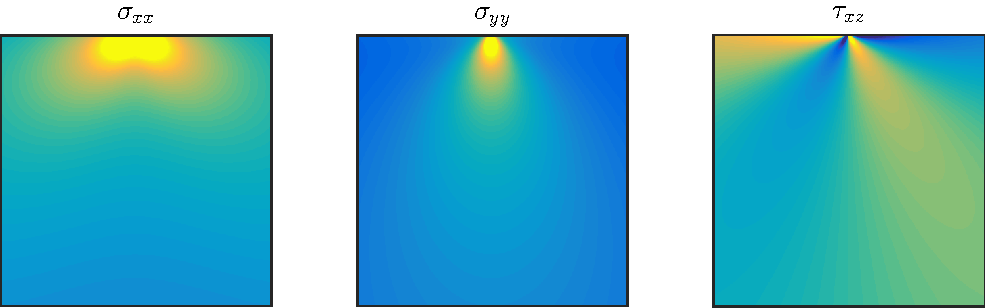
\includegraphics[width=\textwidth]{../figures/thesis/analytic_stress.pdf}
\caption{Near crack-tip stress for a plane crack along the y-axis. The crack tip is located at the top center of each plot.}
\label{fig:analytic_stress}
\end{figure}

